\documentclass[]{book}
\usepackage{lmodern}
\usepackage{amssymb,amsmath}
\usepackage{ifxetex,ifluatex}
\usepackage{fixltx2e} % provides \textsubscript
\ifnum 0\ifxetex 1\fi\ifluatex 1\fi=0 % if pdftex
  \usepackage[T1]{fontenc}
  \usepackage[utf8]{inputenc}
\else % if luatex or xelatex
  \ifxetex
    \usepackage{mathspec}
  \else
    \usepackage{fontspec}
  \fi
  \defaultfontfeatures{Ligatures=TeX,Scale=MatchLowercase}
\fi
% use upquote if available, for straight quotes in verbatim environments
\IfFileExists{upquote.sty}{\usepackage{upquote}}{}
% use microtype if available
\IfFileExists{microtype.sty}{%
\usepackage{microtype}
\UseMicrotypeSet[protrusion]{basicmath} % disable protrusion for tt fonts
}{}
\usepackage{hyperref}
\hypersetup{unicode=true,
            pdftitle={Documentação do projeto `Execução Orçamentária e Financeira do Governo Federal' (``Projeto Caixa'')},
            pdfauthor={R6 Estatística},
            pdfborder={0 0 0},
            breaklinks=true}
\urlstyle{same}  % don't use monospace font for urls
\usepackage{natbib}
\bibliographystyle{apalike}
\usepackage{longtable,booktabs}
\usepackage{graphicx,grffile}
\makeatletter
\def\maxwidth{\ifdim\Gin@nat@width>\linewidth\linewidth\else\Gin@nat@width\fi}
\def\maxheight{\ifdim\Gin@nat@height>\textheight\textheight\else\Gin@nat@height\fi}
\makeatother
% Scale images if necessary, so that they will not overflow the page
% margins by default, and it is still possible to overwrite the defaults
% using explicit options in \includegraphics[width, height, ...]{}
\setkeys{Gin}{width=\maxwidth,height=\maxheight,keepaspectratio}
\IfFileExists{parskip.sty}{%
\usepackage{parskip}
}{% else
\setlength{\parindent}{0pt}
\setlength{\parskip}{6pt plus 2pt minus 1pt}
}
\setlength{\emergencystretch}{3em}  % prevent overfull lines
\providecommand{\tightlist}{%
  \setlength{\itemsep}{0pt}\setlength{\parskip}{0pt}}
\setcounter{secnumdepth}{5}
% Redefines (sub)paragraphs to behave more like sections
\ifx\paragraph\undefined\else
\let\oldparagraph\paragraph
\renewcommand{\paragraph}[1]{\oldparagraph{#1}\mbox{}}
\fi
\ifx\subparagraph\undefined\else
\let\oldsubparagraph\subparagraph
\renewcommand{\subparagraph}[1]{\oldsubparagraph{#1}\mbox{}}
\fi

%%% Use protect on footnotes to avoid problems with footnotes in titles
\let\rmarkdownfootnote\footnote%
\def\footnote{\protect\rmarkdownfootnote}

%%% Change title format to be more compact
\usepackage{titling}

% Create subtitle command for use in maketitle
\providecommand{\subtitle}[1]{
  \posttitle{
    \begin{center}\large#1\end{center}
    }
}

\setlength{\droptitle}{-2em}

  \title{Documentação do projeto `Execução Orçamentária e Financeira do Governo Federal' (``Projeto Caixa'')}
    \pretitle{\vspace{\droptitle}\centering\huge}
  \posttitle{\par}
    \author{R6 Estatística}
    \preauthor{\centering\large\emph}
  \postauthor{\par}
      \predate{\centering\large\emph}
  \postdate{\par}
    \date{2019-12-26}

\usepackage{booktabs}
\usepackage{amsthm}
\makeatletter
\def\thm@space@setup{%
  \thm@preskip=8pt plus 2pt minus 4pt
  \thm@postskip=\thm@preskip
}
\makeatother

\begin{document}
\maketitle

{
\setcounter{tocdepth}{1}
\tableofcontents
}
\hypertarget{introduuxe7uxe3o}{%
\chapter{Introdução}\label{introduuxe7uxe3o}}

\hypertarget{primeiras-instruuxe7uxf5es-do-tiago}{%
\section{Primeiras Instruções do Tiago}\label{primeiras-instruuxe7uxf5es-do-tiago}}

A ideia deste projeto é analisar o comportamento do caixa e das obrigações financeiras dos órgãos federais, com a finalidade de fornecer informações para a gestão da programação financeira por parte do Tesouro Nacional, além de identificar oportunidades de melhorias nesse processo, e possivelmente fundamentar a criação de indicadores para avaliação da gestão financeira das unidades do Governo Federal.

Vamos elencar aqui alguns aspectos, ou componentes, importantes do projeto, sem uma ordem específica.

\hypertarget{uxe9-preciso-de-inuxedcio-conhecer-o-perfil-das-despesas-e-receitas-oruxe7amentuxe1rias-desses-uxf3rguxe3os.}{%
\section{É preciso de início conhecer o perfil das despesas e receitas orçamentárias desses órgãos.}\label{uxe9-preciso-de-inuxedcio-conhecer-o-perfil-das-despesas-e-receitas-oruxe7amentuxe1rias-desses-uxf3rguxe3os.}}

Vamos começar com um perfil das despesas do Ministério da Justiça (que já tem um excelente sistema de acompanhamento das despesas).

\textbf{Tentar compatibilizar as informações orçamentárias (classificações como função, subfunção, ação, grupo de despesa, indicadores orçamentários etc.) com as informações financeiras (vinculação de pagamento, essencialmente).}

O que estamos chamando de \emph{classificadores orçamentários}: Função, Subfunção, Programa, Ação, Grupo de Despesa, Modalidade de Aplicação, Elemento de Despesa, Indicador de Resultado EOF, Indicador de Exceção Decreto.

O que estamos chamando de \emph{classificadores financeiros}: Vinculação de Pagamento, essencialmente.

A \emph{fonte de recurso} é um caso especial, é um classificador comum a esses dois contextos, orçamentário e financeiro.

\hypertarget{como-fazer-isso-diretamente-a-partir-do-siafi}{%
\section{Como fazer isso diretamente a partir do Siafi?}\label{como-fazer-isso-diretamente-a-partir-do-siafi}}

Algumas ideias, a serem testadas:

\begin{itemize}
\item
  analisar as despesas pagas, pelos classificadores, pelo número da nota de empenho e pelo número do documento de pagamento; e relacionar documento de pagamento x nota de empenho x vinculação de pagamento pelo campo ``inscrição'' do documento de pagamento.
\item
  analisar as despesas pagas, pelos classificadores, pelo número da nota de empenho e pelo número do documento de pagamento; e tentar compatibilizar com as informações dos pagamentos efetuados, por vinculação de pagamento e número do documento de pegamento.
\item
  Mais simples: parecido com o anterior, a partir da tabela com as despesas pagas detalhadas pelos classificadores orçamentários, empenho e documento de pagamento, buscar a \emph{vinculação de pagamento} de uma tabela com toda a movimentação do limite de saque detalhada por documento. Assim, quando a movimentação do limite de saque for um pagamento, o documento correspondente, um documento de pagamento, pode ser usado como chave para relacionar as duas tabelas.
\end{itemize}

Teríamos então três extrações: uma para a movimentação no caixa e outras duas, semelhantes em termos de detalhamentos, para os pagamentos totais e para as obrigações a pagar. A relação dos campos está simplificada, e os campos \textbf{destacados} são aqueles que só aparecem na tabela 1, ou que só aparecem nas tabelas 2 e 3.

\hypertarget{movimentauxe7uxf5es-diuxe1rias-do-limite-de-saque-item-de-informauxe7uxe3o-limites-de-saque}{%
\subsection{Movimentações diárias do Limite de Saque (item de informação: ``LIMITES DE SAQUE'')}\label{movimentauxe7uxf5es-diuxe1rias-do-limite-de-saque-item-de-informauxe7uxe3o-limites-de-saque}}

\begin{itemize}
\tightlist
\item
  Órgão Máximo
\item
  Órgão
\item
  UG
\item
  \textbf{Vinculação de Pagamento}
\item
  Fonte Detalhada
\item
  Fonte (posições 3 e 4 da fonte detalhada -- exemplo: se a fonte detalhada é: \texttt{0100123456}, a fonte será \texttt{00})
\item
  Documento Lançamento {[}chave para fazer a junção com tabela (2){]}
\item
  Movimento / Valor Financeiro
\end{itemize}

\hypertarget{pagamentos-diuxe1rios-item-de-informauxe7uxe3o-pagamentos-totais}{%
\subsection{Pagamentos diários (item de informação: ``PAGAMENTOS TOTAIS'')}\label{pagamentos-diuxe1rios-item-de-informauxe7uxe3o-pagamentos-totais}}

\begin{itemize}
\tightlist
\item
  Órgão Máximo
\item
  Órgão
\item
  UG
\item
  Fonte Detalhada
\item
  Fonte (posições 3 e 4 da fonte detalhada -- exemplo: se a fonte detalhada é: \texttt{0100123456}, a fonte será \texttt{00})
\item
  \textbf{Função}
\item
  \textbf{Subfunção}
\item
  \textbf{Programa}
\item
  \textbf{Ação}
\item
  \textbf{Grupo de Despesa}
\item
  \textbf{Modalidade de Aplicação}
\item
  \textbf{Elemento de Despesa}
\item
  \textbf{Indicador de Resultado EOF} (indica se a despesa é primária ou financeira, entre outras coisas)
\item
  \textbf{Indicador de Exceção Decreto}
\item
  \textbf{Ano do Empenho}
\item
  \textbf{Empenho}
\item
  \textbf{Órgão Máximo da UO} (o ``dono'' original do orçamento, que pode ter sido em algum momento ``descentralizado'', isto é, transferido, para um óutro ``Órgão Máximo'' -- ou seja, se o Órgão Máximo da UO é diferente do Órgão Máximo, significa que a unidade está realizando uma despesa com orçamento de outro órgão)
\item
  Documento Lançamento {[}chave para fazer a junção com tabela (1){]}
\item
  Movimento / Valor Financeiro
\end{itemize}

\hypertarget{movimentauxe7uxf5es-diuxe1rias-em-obrigauxe7uxf5es-a-pagar-item-de-informauxe7uxe3o-valores-liquidados-a-pagar-exercicio-rp}{%
\subsection{Movimentações diárias em obrigações a pagar (item de informação: ``VALORES LIQUIDADOS A PAGAR (EXERCICIO + RP)'')}\label{movimentauxe7uxf5es-diuxe1rias-em-obrigauxe7uxf5es-a-pagar-item-de-informauxe7uxe3o-valores-liquidados-a-pagar-exercicio-rp}}

\begin{itemize}
\tightlist
\item
  Órgão Máximo
\item
  Órgão
\item
  UG
\item
  Fonte Detalhada
\item
  Fonte (posições 3 e 4 da fonte detalhada -- exemplo: se a fonte detalhada é: \texttt{0100123456}, a fonte será \texttt{00})
\item
  \textbf{Função}
\item
  \textbf{Subfunção}
\item
  \textbf{Programa}
\item
  \textbf{Ação}
\item
  \textbf{Grupo de Despesa}
\item
  \textbf{Modalidade de Aplicação}
\item
  \textbf{Elemento de Despesa}
\item
  \textbf{Indicador de Resultado EOF} (indica se a despesa é primária ou financeira, entre outras coisas)
\item
  \textbf{Indicador de Exceção Decreto}
\item
  \textbf{Ano do Empenho}
\item
  \textbf{Empenho}
\item
  \textbf{Órgão Máximo da UO} (o ``dono'' original do orçamento, que pode ter sido em algum momento ``descentralizado'', isto é, transferido, para um óutro ``Órgão Máximo'' -- ou seja, se o Órgão Máximo da UO é diferente do Órgão Máximo, significa que a unidade está realizando uma despesa com orçamento de outro órgão)
\item
  Documento Lançamento (acho que não será necessário)
\item
  Movimento / Valor Financeiro
\end{itemize}

\hypertarget{o-que-analisar}{%
\section{O que analisar?}\label{o-que-analisar}}

Com \textbf{(1)} e \textbf{(3)} podemos obter os saldos diários do caixa (tabela \textbf{(1)}) e das obrigações a pagar (tabela \textbf{(3)}) -- e calcular a \emph{disponibilidade líquida diária}, como sendo o saldo do caixa (item ``LIMITES DE SAQUE'') subtraído das obrigações a pagar (item ``VALORES LIQUIDADOS A PAGAR (EXERCICIO + RP)'')--, para cada unidade gestora ou órgão, e para cada fonte de recursos. Para isso sumarizaríamos os dados por DIA\_LANC, UG, ORGAO, FONTE e ITEM\_INFORMACAO. Essa seria a tabela \textbf{(i)}.

Com \textbf{(1)} e \textbf{(2)} poderíamos relacionar, no contexto dos pagamentos, as informações orçamentárias com as vinculações de pagamento, obtendo uma tabela \textbf{(ii)}. Partiríamos de \textbf{(2)} e faríamos um join com \textbf{(1)}, por ``Documento de Lançamento'', para trazer a ``Vinculação de Pagamento'' da tabela \textbf{(1)} (acho que seria interessante trazer também o campo de Movimento / Valor da tabela \textbf{(1)}, porque pode acontecer de um mesmo pagamento ter utilizado mais de uma \emph{vinculação de pagamento}. Nesse caso, o valor mostrado na tabela \textbf{(2)} seria o valor consolidado, e precisaríamos do ).

Finalmente com \textbf{(1)}, podemos analisar as movimentações para tipo de documento, obtendo um histórico das movimentações de cada órgão e cada UG, a que chamaremos de \textbf{(iii)}.

\hypertarget{questuxf5es-iniciais-a-serem-investigadas}{%
\section{Questões iniciais a serem investigadas}\label{questuxf5es-iniciais-a-serem-investigadas}}

\begin{enumerate}
\def\labelenumi{\alph{enumi}.}
\tightlist
\item
  Qual o comportamento do caixa e das obrigações a pagar (e da disponibilidade líquida) no período analisado? Por órgão? Por unidade? Por fonte? Por unidade e por fonte? (Tabela (i))
\end{enumerate}

(semelhante ao que foi feito superficialmente \href{https://github.com/TesouroNacional/puddles-puddles}{aqui}, só que melhor, com mais rigor.)

a1. Há casos em que unidades de um mesmo órgão permanecem com disponibilidade líquida negativa, enquanto outras unidades desse mesmo órgão estão com disponibilidade positiva? E se levarmos em consideração a fonte de recursos, há casos em que o órgão passa por períodos com disponibilidade negativa numa fonte, enquanto há recursos disponíveis em outra fonte? E se levarmos em consideração as duas coisas (unidade + fonte: ou seja, uma unidade de um mesmo órgão fica com disponibilidade negativa numa fonte, enquanto outra unidade desse mesmo órgão possui disponibilidade positiva nessa mesma fonte?)

\begin{enumerate}
\def\labelenumi{\alph{enumi}.}
\setcounter{enumi}{1}
\item
  A partir de (ii), como as classificações orçamentárias se relacionam com as classificações financeiras? Especificamente, é possível identificar certos tipos de despesas que são sempre (ou frequentemente) pagas com recursos de determinadas vinculações?
\item
  Se for possível a identificação mencionada em (b), então, poderíamos fazer uma versão de (i) em que os dados estariam detalhados também por \emph{vinculação de pagamento} e alguns \emph{classificadores orçamentários}. Com o resultado de (b), poderíamos então refinar (a) e (a1), estimando a disponibilidade líquida para cada vinculação, considerando as classificações orçamentárias das obrigações. Por exemplo, a unidade pode ter saldo suficiente para cobrir todas as suas obrigações; mas, quando se analisam na prática que vinculações costumam pagar que obrigações (algo obtido de (b)), pode-se observar que na verdade há suficiência em algumas vinculações, mas insuficiência em outras.
\item
  Qual o comportamento do caixa das unidades, em termos de movimentações? Para isso, podemos considerar os seguintes tipos de movimentações (sete, por enquanto), de acordo com o sinal do valor da movimentação, e do tipo do documento de lançamento (posições 16 e 17 do campo \texttt{ID\_DOCUMENTO}):
\end{enumerate}

\begin{itemize}
\tightlist
\item
  Receitas próprias - movimentos positivos por RAs;
\item
  Recebimentos de recursos financeiros - movimentos positivos por PFs;
\item
  Anulações de pagamentos - movimentos positivos por DF, DR, GF, GP, GR ou OB;
\item
  Ajustes contábeis - movimentos por NS;
\item
  Pagamentos - movimentos negativos por DF, DR, GF, GP, GR ou OB;
\item
  Ajustes na receita arrecadada (anulações, retificações etc.): movimentos negativos por RA; e
\item
  Liberações de recursos para outros órgãos - movimentos negativos por PFs.
\end{itemize}

\begin{enumerate}
\def\labelenumi{\alph{enumi}.}
\setcounter{enumi}{4}
\tightlist
\item
  Provavelmente vamos observar grandes recebimentos de recursos financeiros seguidos por grandes despesas. Nesses casos, em geral, qual o intervalo entre essas duas operações?
\end{enumerate}

\hypertarget{inspirauxe7uxf5es}{%
\section{Inspirações}\label{inspirauxe7uxf5es}}

NatGeo immigrations. Pode ser interessante fazer algo semelhante para visualizar e comparar o saldo diário das unidades.

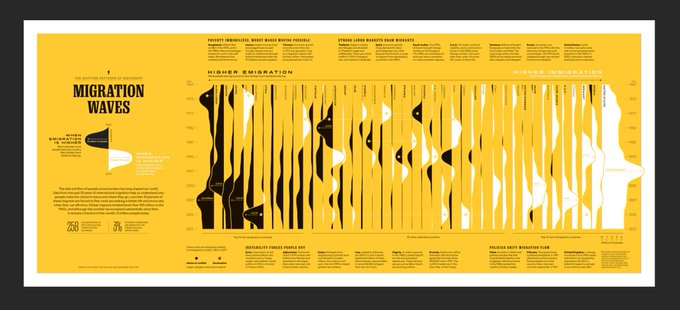
\includegraphics{natgeo.jpg}

\url{https://twitter.com/aLucasLopez/status/1153646875427385344?s=20}

Para mostrar a composição das despesas, vamos usar um diagrama de bolhas em D3 semelhante \href{https://vallandingham.me/bubble_charts_with_d3v4.html}{ao do Jim Vallandingham}.

\hypertarget{bases-de-dados}{%
\chapter{Bases de dados}\label{bases-de-dados}}

\hypertarget{relatuxf3rio-1-validauxe7uxe3o-e-compreensuxe3o-dos-dados}{%
\chapter{Relatório 1: Validação e Compreensão dos Dados}\label{relatuxf3rio-1-validauxe7uxe3o-e-compreensuxe3o-dos-dados}}

\hypertarget{introduuxe7uxe3o-1}{%
\section{Introdução}\label{introduuxe7uxe3o-1}}

A base de dados do SIAFI concentra as informações geradas pelo processo de execução orçamentária e programação financeira do Governo Federal. Este projeto tem como objetivo gerar conhecimento sobre o comportamento do caixa e das obrigações financeiras dos órgãos federais para fins de gestão da programação financeira por parte do Tesouro Nacional, além de identificar oportunidades de melhorias nesse processo e, possivelmente, fundamentar a criação de indicadores para avaliação da gestão financeira das unidades do Governo Federal.

Este é o primeiro dos quatro relatórios que irão compor o projeto e descreve o processo de conhecimento, ajuste e preparo das bases de dados para análises subsequentes.

\hypertarget{questuxf5es-elementares}{%
\section{Questões elementares}\label{questuxf5es-elementares}}

Para nortear as análises das próximas etapas, nessa primeira fase de conhecimento do problema e da base, foram levantadas as seguintes questões:

\begin{enumerate}
\def\labelenumi{\alph{enumi}.}
\item
  Qual o comportamento do caixa e das obrigações a pagar (e da disponibilidade líquida) no período analisado\footnote{Por órgão, por unidade e por fonte de recursos.}?
\item
  Existem casos em que unidades de um mesmo órgão permanecem com disponibilidade líquida negativa, enquanto outras unidades desse mesmo órgão encontram-se com disponibilidade positiva? E se considerar a fonte de recursos, há casos em que o órgão passa por períodos com disponibilidade negativa em uma fonte enquanto há recursos disponíveis em outra fonte? E se considerar as duas situações conjuntamente\footnote{Ou seja, uma unidade de um mesmo órgão fica com disponibilidade negativa em uma fonte, enquanto outra unidade desse mesmo órgão possui disponibilidade positiva nessa mesma fonte.}?
\item
  Como as classificações orçamentárias se relacionam com as classificações financeiras? Especificamente, é possível identificar certos tipos de despesas que são sempre (ou frequentemente) pagas com recursos de determinadas vinculações?
\item
  Caso seja possível a identificação mencionada em (c), as questões (a) e (b) seriam revisitadas para estimar a disponibilidade líquida para cada vinculação, considerando as classificações orçamentárias das obrigações. Nesse cenário, existem unidades com saldo total suficiente para cobrir todas as suas obrigações, porém com insuficiência em algumas vinculações?
\item
  Qual o comportamento do caixa das unidades em termos de movimentações?
\item
  Qual o intervalo entre duas operações\footnote{Uma despesa alta seguida de um recebimento de recursos também alto.} de grande porte?
\end{enumerate}

\hypertarget{bases-de-dados-levantadas-para-endereuxe7ar-as-questuxf5es}{%
\section{Bases de dados levantadas para endereçar as questões}\label{bases-de-dados-levantadas-para-endereuxe7ar-as-questuxf5es}}

O perfil das despesas do \textbf{Ministério da Justiça} será utilizado como ponto de partida das análises descritivas e exploratórias. A escolha deste órgão foi em virtude do seu excelente sistema de acompanhamento das despesas.

Ao todo, três bases foram extraídas:

\begin{itemize}
\tightlist
\item
  \texttt{lim\_saque} com as movimentações de limites de saque;
\item
  \texttt{obrigacoes} com as movimentações de obrigações a pagar; e
\item
  \texttt{pagamentos} com as movimentações de pagamentos;
\end{itemize}

A partir destas, outras três tabelas derivadas foram construídas. As descrições detalhadas estão na seção seguinte.

\begin{itemize}
\item
  \texttt{disponibilidades\_liquidas\_diarias} com as informações diárias de \textbf{saldo disponível} e \textbf{obrigações a pagar} de cada UG para cada fonte de recursos;
\item
  \texttt{vinculacao\_de\_pagamentos} com informações diárias pareadas de \textbf{pagamentos}, \textbf{saldo disponível} e \textbf{vinculações de pagamentos} de cada documento;
\item
  \texttt{lim\_saque\_por\_tipo\_de\_documento} com as informações diárias de \textbf{saldo disponível} por tipo de documento (e.g.~NS, OB, PF, etc.).
\end{itemize}

Verificou-se que as extrações \textbf{encontram-se prontas para análise} e com replicações em formatos \texttt{.rds} para serem leitas pelo software R. Abaixo estão listados os seus respectivos campos.

\hypertarget{base-1-movimentauxe7uxf5es-diuxe1rias-do-limite-de-saque}{%
\section{Base 1: Movimentações diárias do Limite de Saque}\label{base-1-movimentauxe7uxf5es-diuxe1rias-do-limite-de-saque}}

\textbf{Filtro:} item de informação ``LIMITES DE SAQUE''.

\textbf{Campos:}

\begin{itemize}
\tightlist
\item
  Órgão Máximo
\item
  Órgão
\item
  UG
\item
  \textbf{Vinculação de Pagamento}
\item
  Fonte de Recursos Detalhada
\item
  Fonte de Recursos
\item
  Documento Lançamento
\item
  Movimento / Valor Financeiro
\end{itemize}

\hypertarget{base-2-pagamentos-diuxe1rios}{%
\section{Base 2: Pagamentos diários}\label{base-2-pagamentos-diuxe1rios}}

\textbf{Filtro:} item de informação ``PAGAMENTOS TOTAIS''.

\textbf{Campos:}

\begin{itemize}
\tightlist
\item
  Órgão Máximo
\item
  Órgão
\item
  UG
\item
  Fonte de Recursos Detalhada
\item
  Fonte de Recursos
\item
  \textbf{Função}
\item
  \textbf{Subfunção}
\item
  \textbf{Programa}
\item
  \textbf{Ação}
\item
  \textbf{Grupo de Despesa}
\item
  \textbf{Modalidade de Aplicação}
\item
  \textbf{Elemento de Despesa}
\item
  \textbf{Indicador de Resultado EOF} (indica se a despesa é primária ou financeira, entre outras coisas)
\item
  \textbf{Indicador de Exceção Decreto}
\item
  \textbf{Ano do Empenho}
\item
  \textbf{Empenho}
\item
  \textbf{Órgão Máximo da UO}
\item
  Documento Lançamento
\item
  Movimento / Valor Financeiro
\end{itemize}

\hypertarget{base-3-movimentauxe7uxf5es-diuxe1rias-em-obrigauxe7uxf5es-a-pagar}{%
\section{Base 3: Movimentações diárias em obrigações a pagar}\label{base-3-movimentauxe7uxf5es-diuxe1rias-em-obrigauxe7uxf5es-a-pagar}}

\textbf{Filtro:} item de informação ``VALORES LIQUIDADOS A PAGAR (EXERCICIO + RP)''.

\textbf{Campos:}

\begin{itemize}
\tightlist
\item
  Órgão Máximo
\item
  Órgão
\item
  UG
\item
  Fonte Detalhada
\item
  Fonte (posições 3 e 4 da fonte detalhada -- exemplo: se a fonte detalhada é: \texttt{0100123456}, a fonte será \texttt{00})
\item
  \textbf{Função}
\item
  \textbf{Subfunção}
\item
  \textbf{Programa}
\item
  \textbf{Ação}
\item
  \textbf{Grupo de Despesa}
\item
  \textbf{Modalidade de Aplicação}
\item
  \textbf{Elemento de Despesa}
\item
  \textbf{Indicador de Resultado EOF} (indica se a despesa é primária ou financeira, entre outras coisas)
\item
  \textbf{Indicador de Exceção Decreto}
\item
  \textbf{Ano do Empenho}
\item
  \textbf{Empenho}
\item
  \textbf{Órgão Máximo da UO}
\item
  Movimento / Valor Financeiro
\end{itemize}

\hypertarget{tabelas-derivadas}{%
\section{Tabelas Derivadas}\label{tabelas-derivadas}}

\hypertarget{disponibilidades-luxedquidas-diuxe1rias}{%
\subsection{Disponibilidades líquidas Diárias}\label{disponibilidades-luxedquidas-diuxe1rias}}

\begin{itemize}
\item
  Informações diárias de \textbf{saldo disponível} e \textbf{obrigações a pagar} de cada UG para cada fonte de recursos.
\item
  Útil para as questões \textbf{a}, \textbf{c} e \textbf{e}.
\item
  Cruzamento entre as bases \texttt{lim\_saque} e \texttt{obrigacoes} pelas chaves \texttt{NO\_DIA\_COMPLETO}, \texttt{NO\_FONTE\_RECURSO} e \texttt{NO\_UG}.
\item
  Observações: 352.037
\item
  Campos: 11
\end{itemize}

\begin{verbatim}
* NO_DIA_COMPLETO         `<date> 2017-08-22, 2017-08-23, 2017-08-24, 2017-08…`
* NO_UG                   `<chr> "ACADEMIA NACIONAL DA POLICIA RODOV. FEDERAL…`
* NO_ORGAO                `<chr> "DEPARTAMENTO DE POLICIA RODOVIARIA FEDERAL/…`
* NO_FONTE_RECURSO        `<chr> "RECEITAS DE CONCURSOS DE PROGNOSTICOS", "RE…`
* saldo_diario            `<dbl> -2779.98, -5654.96, -7356.26, -5601.60, -560…`
* obrigacoes_a_pagar      `<dbl> 0.000000e+00, 0.000000e+00, 0.000000e+00, 0.…`
* disponibilidade_liquida `<dbl> -2779.98, -5654.96, -7356.26, -5601.60, -560…`
* ano                     `<dbl> 2017, 2017, 2017, 2017, 2017, 2017, 2017, 20…`
* mes                     `<dbl> 8, 8, 8, 8, 8, 8, 8, 8, 8, 8, 9, 9, 9, 9, 9,…`
* dia                     `<int> 22, 23, 24, 25, 26, 27, 28, 29, 30, 31, 1, 2…`
* paded                   `<lgl> TRUE, TRUE, TRUE, TRUE, FALSE, FALSE, TRUE, …`
\end{verbatim}

\hypertarget{vinculauxe7uxe3o-de-pagamentos}{%
\subsection{Vinculação de Pagamentos}\label{vinculauxe7uxe3o-de-pagamentos}}

\begin{itemize}
\item
  Informações diárias pareadas de \textbf{pagamentos}, \textbf{saldo disponível} e \textbf{vinculações de pagamentos} de cada documento.
\item
  Útil para as questões \textbf{b}, \textbf{c} e \textbf{e}.
\item
  Cruzamento entre as bases \texttt{lim\_saque} e \texttt{pagamentos} pelas chaves \texttt{NO\_DIA\_COMPLETO} e \texttt{ID\_DOCUMENTO}.
\item
  Observações: 1.005.187
\item
  Campos: 7
\end{itemize}

\begin{verbatim}
* NO_DIA_COMPLETO         `<chr> "01/02/2017", "01/02/2017", "01/02/2017", "0…`
* ID_DOCUMENTO            `<chr> "194003192082017OB800016", "194003192082017O…`
* pagamento               `<dbl> 20.79, 724.21, 8000.00, 76.95, -15188.99, -9…`
* NO_VINCULACAO_PAGAMENTO `<chr> "CUSTEIO/INVESTIMENTO - RESUL.PRIM = 2", "CU…`
* vinculacoes_distintas   `<int> 1, 1, 1, 1, 1, 1, 1, 1, 1, 1, 1, 1, 1, 1, 1,…`
* saldo_diario            `<dbl> -20.79, -724.21, -8000.00, -76.95, 15188.99,…`
* pagamento_por_saldo     `<dbl> -1, -1, -1, -1, -1, -1, -1, -1, -1, -1, -1, …`
\end{verbatim}

\hypertarget{limimtes-de-saque-por-tipo-de-documento}{%
\subsection{Limimtes de Saque Por Tipo De Documento}\label{limimtes-de-saque-por-tipo-de-documento}}

\begin{itemize}
\item
  Informações diárias de \textbf{saldo disponível} por tipo de documento. Os tipos de documentos são: \texttt{DF}, \texttt{DR}, \texttt{GF}, \texttt{GP}, \texttt{GR}, \texttt{NL}, \texttt{NS}, \texttt{OB}, \texttt{PF} e \texttt{RA}.
\item
  Útil para a questão \textbf{d}.
\item
  Derivada da base \texttt{lim\_saque}.
\item
  Observações: 254.667
\item
  Campos: 7
\end{itemize}

\begin{verbatim}
* tipo_de_documento  `<chr> "DF", "DF", "DF", "DF", "DF", "DF", "DF", "DF", "…`
* NO_DIA_COMPLETO    `<chr> "01/02/2017", "01/02/2017", "01/02/2017", "01/02/…`
* NO_UG              `<chr> "COORD. REG. NOROESTE DO MATO GROSSO/MT", "COORDE…`
* NO_ORGAO           `<chr> "FUNDACAO NACIONAL DO INDIO", "DEPARTAMENTO DE PO…`
* NO_ITEM_INFORMACAO `<chr> "LIMITES DE SAQUE (OFSS, DIVIDA, BACEN E PREV)", …`
* NO_FONTE_RECURSO   `<chr> "RECURSOS ORDINARIOS", "RECURSOS ORDINARIOS", "TX…`
* saldo_diario       `<dbl> -35.47, -2089.65, -3644.19, -12.01, -14.94, -31.3…`
\end{verbatim}

\hypertarget{tuxedtulo-a}{%
\chapter{Título A}\label{tuxedtulo-a}}

`r if (knitr:::is\_html\_output()) '
\# Referências \{-\}

\begin{itemize}
\tightlist
\item
  \url{https://www.nature.com/articles/s41598-017-13448-3}
\item
  \url{https://github.com/gm-spacagna/deep-ttf/}
  \textasciitilde{}
\end{itemize}

\bibliography{book.bib,packages.bib}


\end{document}
